\documentclass{beamer}
\usepackage{feynmp} % setup feynmp
\DeclareGraphicsRule{*}{mps}{*}{}
\usepackage{tikz}

% theme and general look
\usetheme{Rochester}
\usecolortheme{seahorse}

\setbeameroption{show notes}

% title information
\title[Muon Production and $A_{FB}$]{Muon Pair Production and Forward-Backward Asymmetry}
\author{L.~Siemens}


\begin{document}
\begin{fmffile}{presentation_mp} % begin feynmp environment

\begin{frame}
    \titlepage
    \note{\tableofcontents}
\end{frame}

\section{Setup}
\subsection{Montecarlo methods}
\begin{frame}{Mathematical Methods: Monte Carlo Integration}
    $$f_{\text{avg}} = \frac{1}{b - a}\int_a^b f(x)dx$$
    Integral converges as $~\frac{1}{\sqrt{N}}$
    \note[item]{Define monte carlo integration and the convergence properties}
\end{frame}

\begin{frame}{Mathematical Methods: Monte Carlo Sampling}{Rejection Sampling}
    \begin{itemize}
        \item Sample (x, v) uniformly from $[a, b]\times[0, 1]$
        \item Reject samples if $\frac{f(x)}{f_{\text{max}}} < v$
    \end{itemize}

    \note[item]{Monte Carlo sampling Goal: produce samples following an
                arbitrary distribution}
    \note[item]{Randomly sample the domain and the interval 0 to 1 (x, v)}
    \note[item]{reject any sample where the function divided by the maximum at x
                is less than the value v}
    \note[item]{The remaining samples will be distributed according to
                the function $f(x)$}
\end{frame}

\subsection{Equations and differential cross section}
\begin{frame}{Muon Pair Production: $e^+ + e^- \rightarrow \mu^+ + \mu^-$}
    equations for the Number of events given the luminosity
    show feynman diagram and collision diagram
    give equations for relevent momentum

    \begin{fmfgraph*}(120, 80)
        \fmfleft{i2,i1}
        \fmfright{o4,o3}
        \fmf{fermion}{i1,v1,i2}
        \fmf{fermion}{o3,v2,o4}
        \fmf{photon, label=$\gamma,,Z^0$}{v1,v2}
        \fmflabel{$e$}{i2}
        \fmflabel{$\mu$}{o4}
        % Momentum arrows
        \fmfcmd{%
            vardef normal (expr p, mag) = 
                (1, 0)
                rotated (90 + angle direction 0.5*length(p) of p)
                scaled mag
            enddef;
            % draw momentum arrow on left side of ray
            style_def marrowl expr p =
                drawarrow subpath (1/4, 3/4) of p
                shifted normal (p, 6)
                withpen pencircle scaled 0.4;
            enddef;
            % draw momentum arrow on right side of ray
            style_def marrowr expr p =
                drawarrow subpath (1/4, 3/4) of p
                shifted normal (p, -6)
                withpen pencircle scaled 0.4;
            enddef;}
        \fmf{marrowl, label=$p_1$, tension=0}{i1,v1}
        \fmf{marrowr, label=$p_3$, tension=0}{v2,o3}
    \end{fmfgraph*}

    \begin{figure}
    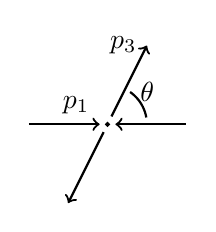
\begin{tikzpicture}
        \draw [thick,->] (-1,0) -- (-0.1,0) node[above left] {$p_1$};
        \draw [thick,<-] (0.1,0) -- (1,0);
        \draw [thick,->] (0.05,0.1) -- (0.5,1) node[left] {$p_3$};
        \draw [thick,domain=10:55] plot ({0.5*cos(\x)}, {0.5*sin(\x)}) node[right] {$\theta$};
        \draw [thick,<-] (-0.5,-1) -- (-0.05,-0.1);
        \draw [fill] (0,0) circle [radius=0.025];
    \end{tikzpicture}
    \end{figure}
\end{frame}

\begin{frame}{Differential Cross Section}
    Mention the terms for the two diagrams, the effect of propegators
    the vertex factors for the weak interaction and the effect of decay
    show the relation ship with $cos(\theta)$ and the symmetry/asymmetry
    of the differnt terms.
\end{frame}

\subsection{Simulation Outline}
\begin{frame}{Simulation Outline}
    estimate the total cross section and maximum of the distribution
    estimate the number of events using the luminosity and cross section
    sample a poisson distribution to get spesific number of events
    get that many events following the differential cross section distribution
    calculate the 4-momentum of P3 and save to disk
\end{frame}

\section{The Data}
\subsection{Angular Distribution}
\subsection{Cross Section vs Energy}
\subsection{Forward Backward Asymmetry Equations (Optional?)}
\subsection{Forward Backward Asymmetry}
\begin{frame}
    TODO fill in frames for data and results
    \note[item]{Talk about the $A_{FB}$ asymmetry}
\end{frame}

\end{fmffile}
\end{document}
